\section{}
\subsection{Question}
Given a non-empty integer array, find the minimum number of moves required to make all array elements equal, where a move is incrementing a selected element by 1 or decrementing a selected element by 1.

You may assume the array's length is at most 10,000.

Example:

Input:
[1,2,3]

Output:
2

Explanation:

Only two moves are needed (remember each move increments or decrements one element):

$[1,2,3] => [2,2,3] => [2,2,2]$

Input:

int A[]: the input array.

int N: length of A.

Output:

int minMoves.


\subsection{Answer}
For this problem, it is easy to find that we only need to get the medium number of the array and calculate the sum of the absolute difference between every item and the medium.

The question is to find the medium number of the array. One trivial solution is to sort the array and get the number with index n/2. The time complexity is O(nlogn). Another solution is to get the medium number similar to quick sort. In this solution, the mean time complexity can be O(n).

Use the same method and the function partition of quick sort. The difference is that we use an index to check whether the n/2 index has already set. And stop here.
\textbf{\color{red}Time complexity O(n)}
\newpage
\subsection{Code}
\texttt{C++ :}
\lstinputlisting[breaklines=TRUE,basicstyle=\footnotesize\ttfamily,language=c++,numbers=left, numberstyle=\tiny,keywordstyle=\color{blue},commentstyle=\color{red!50!green!50!blue!50},frame=shadowbox, rulesepcolor=\color{red!20!green!20!blue!20},stringstyle=\color{purple}]{1.cpp}

\newpage
\section{}
\subsection{Question}
Given a string that consists of only uppercase English letters, you can replace any letter in the string with another letter at most k times. Find the length of a longest substring containing all repeating letters you can get after performing the above operations.
    
Note:Both the string's length and k will not exceed $10^4$.

Example:

Input:

s = "AABABBA", k = 1

Output:

4

Explanation:

Replace the one 'A' in the middle with 'B' and form "AABBBBA".
The substring "BBBB" has the longest repeating letters, which is 4.

Input:

string s;

int k;

Output:

return the length of the longest substring.

\subsection{Answer}
We use slide window to solve this problem. The problem says that we can make at most k changes to the string. To convert this problem, for any substring, we can calculate a number (len(substring) - number of maximum character in this substring).  As long as this answer is $\leq k$, this is a good string. And we want to maximize the length of this substring by extending the end length.

Given this, we can maintain a sliding window. First, extend the window to its limit, that is, the longest we can get to with maximum number of modifications. 

Then as end increase, the whole substring disobey the k rule, so we need to move start to the right until the whole string satisfy it again. Every time we need to get the maximum length of the substring.


\textbf{\color{red}Time complexity O($n^2$)}
\subsection{Code}
\texttt{C++ :}
\lstinputlisting[breaklines=TRUE,basicstyle=\footnotesize\ttfamily,language=c++,numbers=left, numberstyle=\tiny,keywordstyle=\color{blue},commentstyle=\color{red!50!green!50!blue!50},frame=shadowbox, rulesepcolor=\color{red!20!green!20!blue!20},stringstyle=\color{purple}]{2.cpp}

\newpage
\section{}
\subsection{Question}
You are given an array x of n positive numbers. You start at point (0,0) and moves x[0] metres to the north, then x[1] metres to the west, x[2] metres to the south, x[3] metres to the east and so on. In other words, after each move your direction changes counter-clockwise.

Write a one-pass algorithm with O(1) extra space to determine, if your path crosses itself, or not.

Example 1:

Given x = [2, 1, 1, 2]

Return true (self crossing)

Example 2:

Given x = [1, 2, 3, 4]

Return false (not self crossing)

Example 3:

Given x = [1, 1, 1, 1]

Return true (self crossing)

Input:

int x[]: the input array.

int N: length of x.

Output:

return true or false.

\subsection{Answer}

At first glance, this problem may be difficult and the code can be complex. However, We can consider when will there be a self cross.

There are in all three situations. The direction changes counter-clockwise. So when the direction changes for 3 4 5 times, there can be a self cross. When there are more changes of direction, they are the same to the previous ones for 360/90=4.

So consider these three situations. Take 3 as an example.
We need to satisfy that 
$x[i]\geq x[i-2] \&\& x[i-1] \leq x[i-3]$, so that there is a cross.
So do the other two situations.

\begin{figure}[H]
\centering
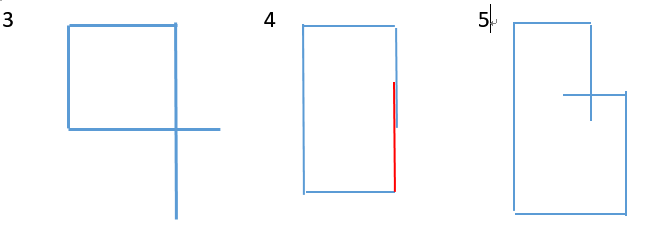
\includegraphics[scale=0.5]{1.png}
\caption{Three situation for self crossing}
\label{hill}
\end{figure}

\textbf{\color{red}Time complexity O(n)}
\newpage
\subsection{Code}
\texttt{C++ :}
\lstinputlisting[breaklines=TRUE,basicstyle=\footnotesize\ttfamily,language=c++,numbers=left, numberstyle=\tiny,keywordstyle=\color{blue},commentstyle=\color{red!50!green!50!blue!50},frame=shadowbox, rulesepcolor=\color{red!20!green!20!blue!20},stringstyle=\color{purple}]{3.cpp}

